\begin{figure}[!t]
\begin{tabular}{c c c}
\begin{minipage}{.45\textwidth}
(a) Human expert approach
\end{minipage}
& &
\begin{minipage}{.45\textwidth}
(b) Filter then Average {\scriptsize \citep{holste2022automated}}
\end{minipage}
\\
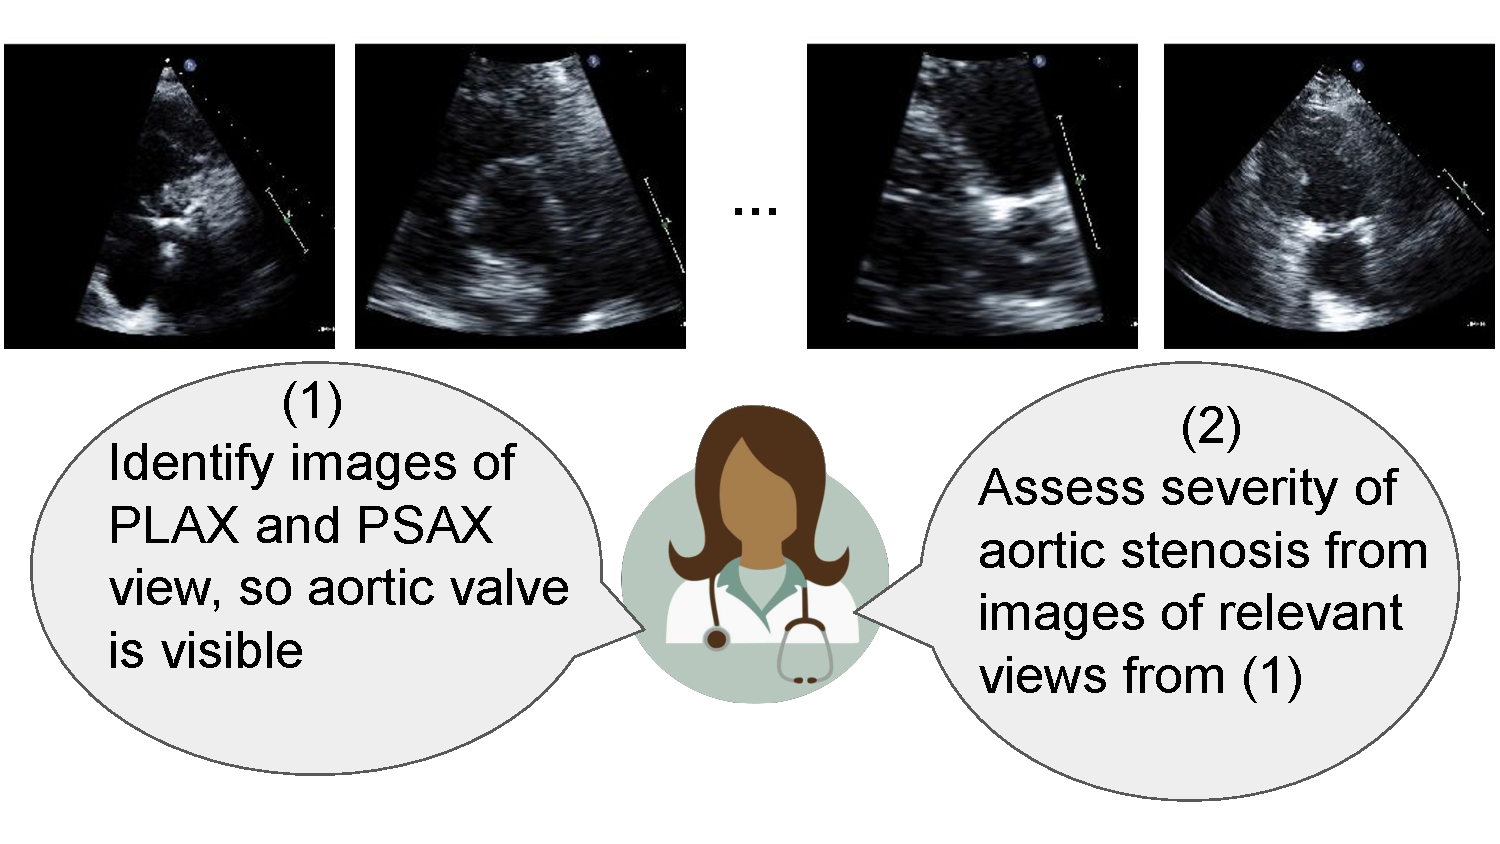
\includegraphics[width=0.45\textwidth]{figures/MIL_for_AS_diagram_1.pdf}
& &
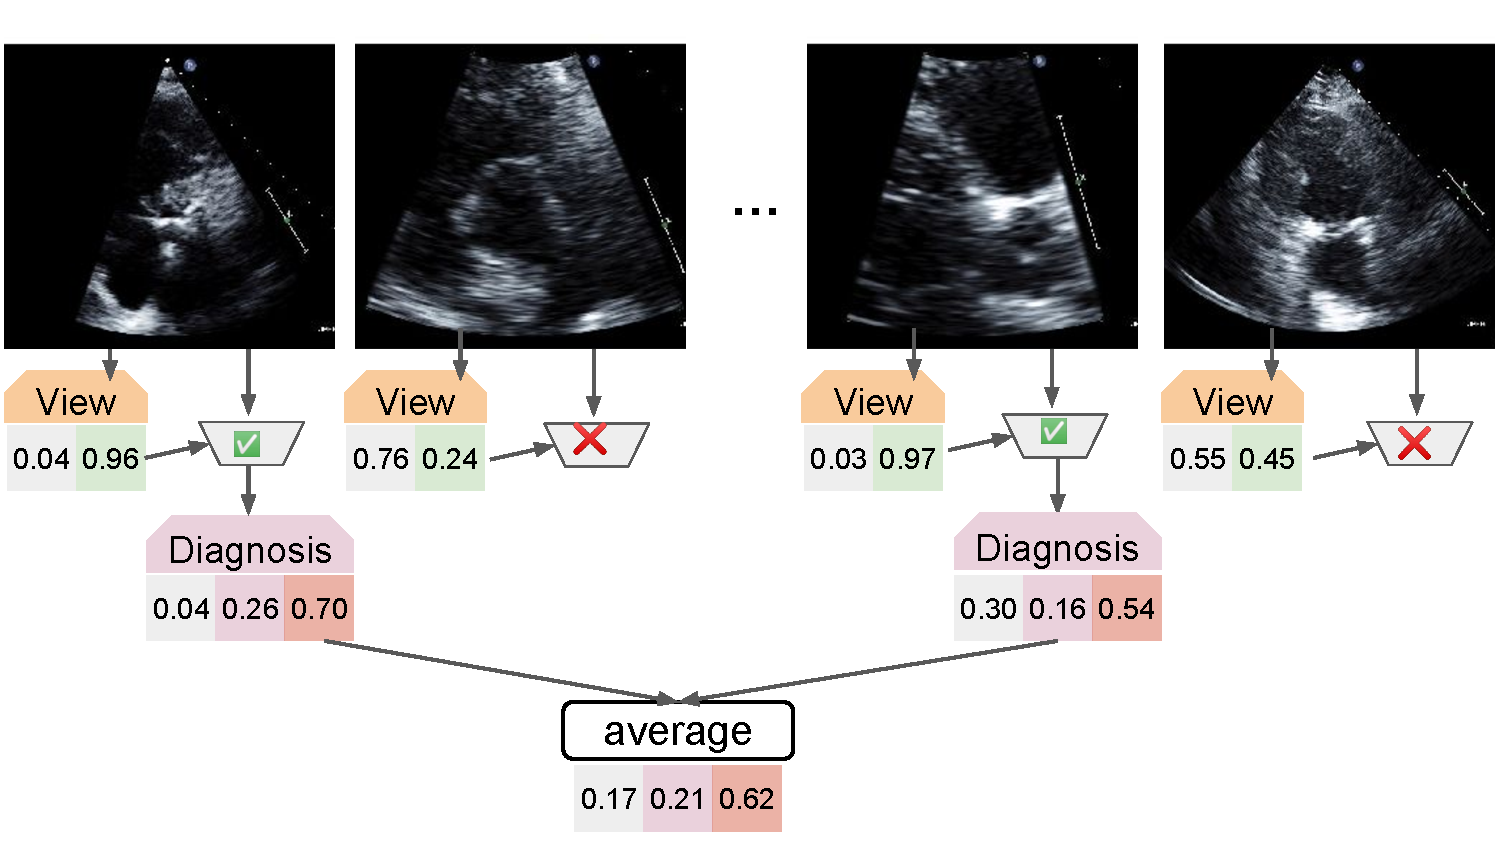
\includegraphics[width=0.45\textwidth]{figures/MIL_for_AS_diagram_2.pdf}
\\
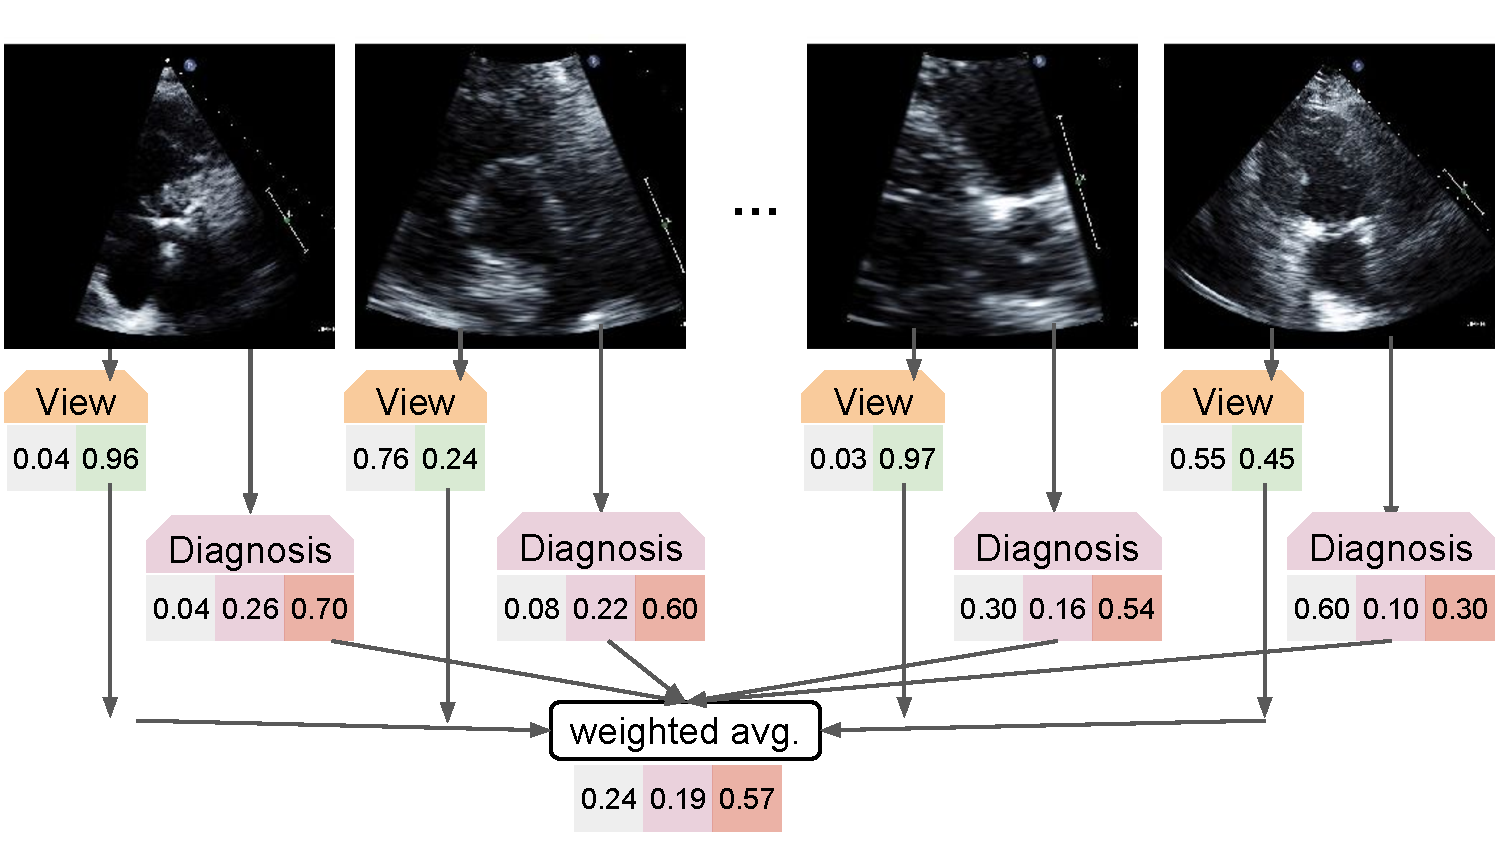
\includegraphics[width=0.45\textwidth]{figures/MIL_for_AS_diagram_3.pdf}
& &
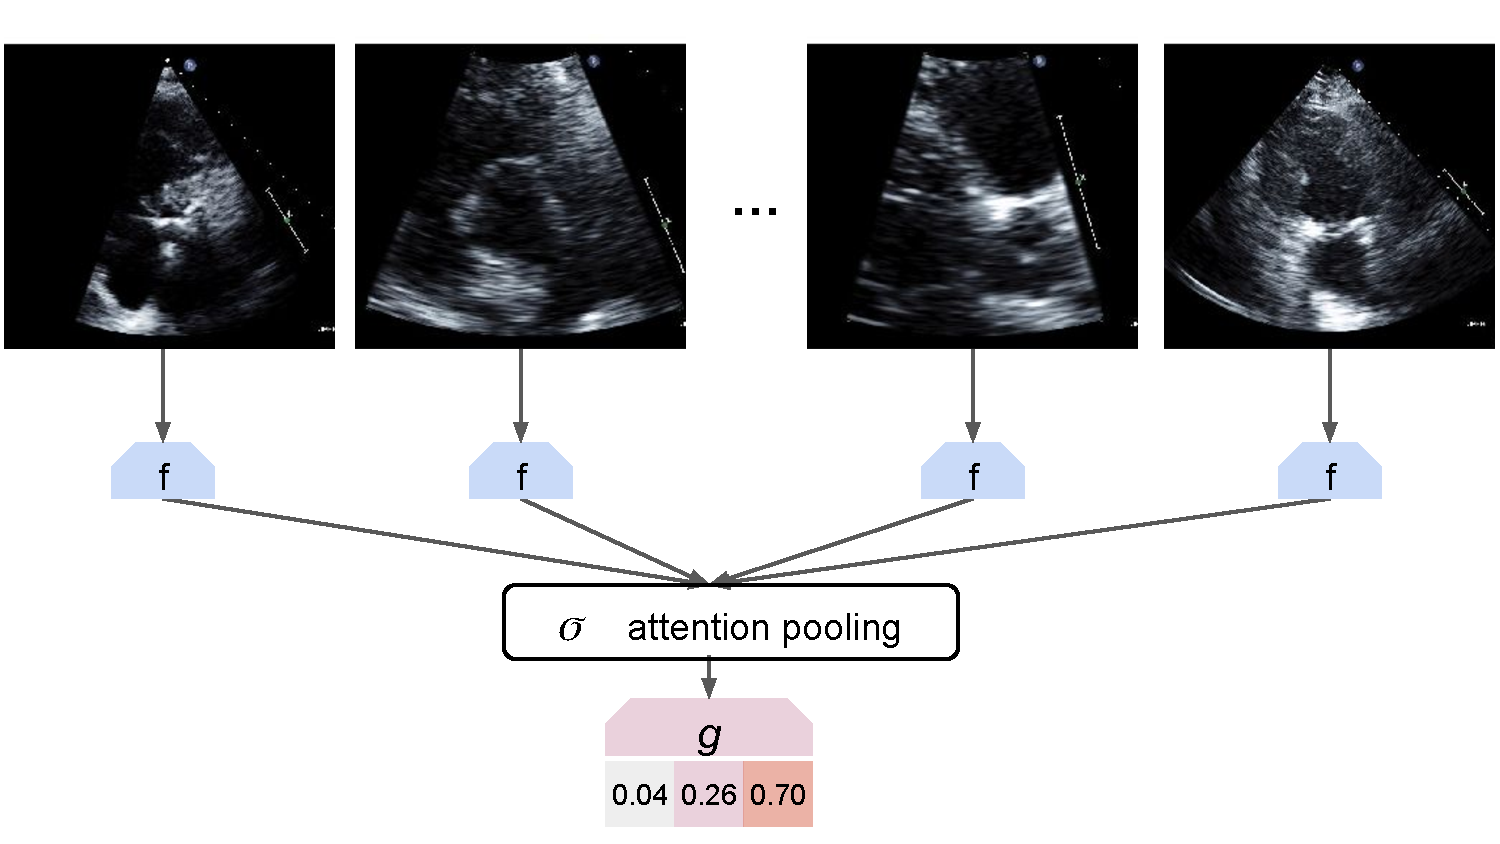
\includegraphics[width=0.45\textwidth]{figures/MIL_for_AS_diagram_4.pdf}
\\
\begin{minipage}{.45\textwidth}
(c) Weighted Average by View Relevance {\scriptsize \citep{wessler2023automated,huang2021new}}
\end{minipage}
& &
\begin{minipage}{.45\textwidth}
(d) Attention-based MIL ~\\
\end{minipage}
\end{tabular}
\caption{\textbf{Overview of methods for diagnosing aortic valve disease from multiple images of the heart.}
In our chosen diagnostic problem, the input is multiple ultrasound images representing different canonical view types of the heart's complex anatomy (e.g. PLAX, PSAX, A2C, A4C, and more, see \citet{mitchell2019guidelines} for a taxonomy).
The required output is a (probabilistic) prediction of the severity of Aortic Stenosis (AS), on a 3-level scale of no / early / significant disease.
We wish to develop deep learning methods that can solve this problem like expert cardiologists (panel a).
Two recent efforts (panel b by others, panel c by our group) made progress using a separately-trained view type classifier and per-image diagnosis classifier, but rely on combining diagnosis probabilities across images via average pooling that cannot learn how to distribute attention non-uniformly among images of relevant views.
In this work, we develop more flexible attention-based multiple instance learning architectures (MIL, panel d), with crucial contributions of supervised attention (Sec.~\ref{sec:methods_SA}) and improved pretraining strategies (Sec.~\ref{sec:methods_CL}) that we show later yield substantially improved performance on this task.
}%endcaption
\label{fig:diagrams}
\end{figure}